% Evidence: thesis Chapters 3--6, Appendix B, and src/switching/conversion.py.
% Keep noframenumbering on every frame; this file is included after \appendix.

\begin{frame}[noframenumbering,label=backup-rules]{B1 | Exact Switch-Conversion Rules}
\small All rules below produce the \textbf{raw binary decision} at time $t$.\par
\vspace{3mm}
\renewcommand{\arraystretch}{1.65}
\begin{tabularx}{\textwidth}{@{}p{30mm}X@{}}
\toprule
Formulation & Activate when\ \ldots\\\midrule
\textcolor{forecast}{Autoregressive} & $\widehat S_{t+k}\geq10$ for every $k=1,\ldots,10$.\\
\textcolor{current}{Current-level} & $S_t\geq10$ and $\widehat R_t^{\mathrm{level}}\geq300\,\mathrm{s}$.\\
\textcolor{longfade}{Long-fade} & $P(D_{\mathrm{event}}\geq300\,\mathrm{s}\mid X_t)\geq0.5$.\\
\textcolor{survival}{Survival} & $S_t\geq10$ and $\widehat{\mathcal S}(300\,\mathrm{s}\mid X_t)\geq0.65$.\\
\bottomrule
\end{tabularx}
\smallnote{$S_t$: current signal in dB. $\mathcal S$: survival probability. The survival threshold 0.65 is exploratory/test-selected, not validation-calibrated.}
\takeaway{Then apply the same short-island extension and above-threshold holding rule.}
\end{frame}


\begin{frame}[noframenumbering]{B2 | Perfect Switch and Post-Processing}
\begin{columns}[T,onlytextwidth]
\column{.48\textwidth}
\begin{block}{An offline reference}
At 30-second sampling, find \textbf{11 consecutive observations} with $S\geq10$ dB. They span ten intervals, or 300 seconds.
\end{block}
\small Mark each qualifying window. Overlapping windows recover the qualifying threshold run.
\vspace{3mm}

The reference sees the true future. It is an \textbf{oracle benchmark}, not a deployable predictor.
\column{.48\textwidth}
\begin{block}{Shared binary post-processing}
\begin{enumerate}
\item Extend each short positive island to ten samples, bounded by its processing group.
\item Hold an active decision while the current signal remains above threshold.
\end{enumerate}
\end{block}
\small This may connect nearby islands; it does \textbf{not} merge every gap or remove short islands.
\end{columns}
\vspace{3mm}
\[
b_t=\begin{cases}1,&b_{t-1}=1\ \text{and}\ S_t\geq10,\\e_t,&\text{otherwise},\end{cases}
\qquad e_t=\text{extended decision}.
\]
\smallnote{Evaluate the held switch, not the legacy adjusted diagnostic. Ten active samples contribute 300 s to active duration.}
\end{frame}

\begin{frame}[noframenumbering]{B3 | Models and Input Representations}
\small
\renewcommand{\arraystretch}{1.45}
\begin{tabularx}{\textwidth}{@{}>{\raggedright\arraybackslash}p{27mm}>{\raggedright\arraybackslash}p{48mm}>{\raggedright\arraybackslash}X@{}}
\toprule
Task & Models & Input variants\\\midrule
\textcolor{forecast}{Autoregressive} & GRU S2V; GRU encoder--decoder; PatchTST; XGBoost & Raw and context-standardized;\newline $L=30$, $h=10$.\\
 & Chronos zero-shot & Raw; $L=30$ and $L=120$; $h=10$.\\
\textcolor{current}{Current-level} & Shapelet MLP, convolution and Transformer; XGBoost & Relative-to-current context plus scalar features.\\
\textcolor{longfade}{Long-fade} & XGBoost; TCN; shapelet convolution & Relative-to-threshold context plus scalar features.\\
\textcolor{survival}{Survival} & XGBoost-AFT; discrete-time TCN & Selected AFT: raw lags. Selected TCN: relative-to-current plus scalars.\\
\bottomrule
\end{tabularx}
\smallnote{Unless noted otherwise, context length is 30 observations. Every input feature comes from Signal history; no meteorological covariates are used.}
\takeaway{Different outputs require different labels, but all decisions are evaluated against Perfect Switch.}
\end{frame}

\begin{frame}[noframenumbering]{B4 | Search Scope and Model Selection}
\small
\renewcommand{\arraystretch}{1.24}
\begin{tabularx}{\textwidth}{@{}Xrr@{}}
\toprule
Search & Trials & Validation criterion\\\midrule
Autoregressive GRU (two architectures, two variants) & 576 & RMSE $\downarrow$\\
Autoregressive PatchTST (two variants) & 1,728 & RMSE $\downarrow$\\
Autoregressive XGBoost (two variants) & 2,304 & RMSE $\downarrow$\\
Current-level shapelets (three heads) & 648 & MAE in seconds $\downarrow$\\
Current-level XGBoost & 1,152 & MAE in seconds $\downarrow$\\
Long-fade (three model families) & 8,928 & AUPRC $\uparrow$\\
Survival XGBoost-AFT & 1,920 & AFT negative log-likelihood $\downarrow$\\
Survival TCN & 1,620 & Integrated Brier score $\downarrow$\\
\bottomrule
\end{tabularx}
\smallnote{Archived grid counts across the included variants. Chronos is zero-shot. The survival TCN grid follows controlled validation experiments on representation, binning and weighting.}
\takeaway{Hyperparameters are selected on validation; refit or checkpoint promotion is recorded in run metadata.}
\end{frame}

\begin{frame}[noframenumbering]{B5 | Normalization and Data Availability}
\begin{columns}[T,onlytextwidth]
\column{.48\textwidth}
\textbf{Context standardization}
\[
\mu_t=\frac{1}{L}\sum_{j=0}^{L-1}S_{t-j},\qquad
\widetilde X_t=\frac{X_t-\mu_t}{s_t}
\]
\small $s_t$ is the context standard deviation, with a numerical safeguard. Targets use the \textbf{same context statistics}.
\[
\widehat Y_t^{\mathrm{raw}}=s_t\widehat Y_t^{\mathrm{standard}}+\mu_t
\]
\small No future-window statistics enter this transformation.
\column{.48\textwidth}
\textbf{Auxiliary scalar features}
\small\par\vspace{3mm}
Past/current signal level, window summaries and slopes; train-fitted feature scaling.
\vspace{5mm}

\textbf{Small-gap reconstruction}\par\vspace{2mm}
Offline linear interpolation: at most two inserted samples in a gap of at most 90 s. Longer gaps separate acquisition segments.
\smallnote{Interpolation can require the right endpoint: an online implementation must account for its availability and latency.}
\end{columns}
\takeaway{An external test source is held out; development splits are chronological and event-aware.}
\end{frame}

\begin{frame}[noframenumbering]{B6 | Event Definitions and Censoring}
\small
\renewcommand{\arraystretch}{1.4}
\begin{tabularx}{\textwidth}{@{}p{29mm}X@{}}
\toprule
Current-level & Search the full continuous signal for the first value below $S_t-0.5$. A local event-window boundary does not terminate the target.\\
Long-fade & Group threshold crossings within three hours of the first crossing. Temporary exits between grouped crossings remain inside the event.\\
Survival & A state machine confirms recovery instead of splitting at every temporary threshold exit. Estimate time to the end of this event.\\
\bottomrule
\end{tabularx}
\vspace{3mm}
\begin{columns}[T,onlytextwidth]
\column{.48\textwidth}
\begin{block}{Observed event end}
Residual duration $R_t$ is known.\par
AFT bounds: $[R_t,R_t]$.
\end{block}
\column{.48\textwidth}
\begin{block}{Acquisition ends first}
Only follow-up $C_t$ is known: $R_t>C_t$.\par
AFT bounds: $[C_t,+\infty)$.
\end{block}
\end{columns}
\smallnote{Survival keeps right-censored samples. Ordinary current-level duration regression excludes them. A later sample across a long gap does not prove continuous persistence.}
\end{frame}

\begin{frame}[noframenumbering]{B7 | Large Duration Error, Correct Switch?}
\small Assume the current signal is already $\geq10$ dB. Compare the duration gate at 300 s:\par
\vspace{4mm}
\renewcommand{\arraystretch}{1.6}
\begin{tabularx}{\textwidth}{@{}Xrrr@{}}
\toprule
Illustrative example & True duration & Prediction & Absolute error\\\midrule
Both above 300 s & 3,600 s & 600 s & \textcolor{alertred}{3,000 s}\\
Opposite sides of 300 s & 310 s & 290 s & \textcolor{current}{20 s}\\
\bottomrule
\end{tabularx}\par
\vspace{4mm}
\begin{columns}[T,onlytextwidth]
\column{.48\textwidth}
\begin{block}{First example}
Large numerical error, but the same threshold decision.
\end{block}
\column{.48\textwidth}
\begin{block}{Second example}
Small numerical error, but the wrong threshold decision.
\end{block}
\end{columns}
\smallnote{Illustrations, not measured samples. Even a correct current-level duration gate is only a proxy for Perfect Switch: current-level recovery is not fade recovery.}
\takeaway{Duration MAE, threshold accuracy and final switch quality answer different questions.}
\end{frame}

\begin{frame}[noframenumbering]{B8 | Native Grid, Reference Grid, Intersection}
\small
\renewcommand{\arraystretch}{1.5}
\begin{tabularx}{\textwidth}{@{}>{\raggedright\arraybackslash}p{29mm}>{\raggedright\arraybackslash}X>{\raggedright\arraybackslash}X@{}}
\toprule
Evaluation domain & What it measures & Main limitation\\\midrule
Native task grid & Decision quality where the task produces predictions. & Different timestamp sets across tasks.\\
Common reference grid & One reference timeline; unavailable decisions map to 0. & Quality and native coverage are combined.\\
Strict intersection & Only timestamps with native decisions from all compared tasks. & Smaller, selected domain: 771 timestamps.\\
\bottomrule
\end{tabularx}\par
\vspace{4mm}
\textbf{Strict-intersection diagnostic: switch F1}\par\vspace{2mm}
Current-level XGBoost: \textbf{0.900}\quad
Survival AFT: \textbf{0.872}\quad
Autoregressive XGBoost raw: \textbf{0.866}
\smallnote{These are not the reference-grid scores on the main slides. Mapping missing decisions to 0 is an evaluation convention, not a validated deployment fallback.}
\takeaway{State the evaluation grid before interpreting a cross-task ranking.}
\end{frame}

\begin{frame}[noframenumbering]{B9 | How the Survival Models Produce Probabilities}
\begin{columns}[T,onlytextwidth]
\column{.48\textwidth}
\textcolor{survival}{\textbf{XGBoost-AFT}}
\[
\log R=f(X)+\tau Z
\]
\small Trees predict a log-time location. A noise distribution and scale $\tau$ define a duration distribution:
\[
\mathcal S(u\mid X)=1-F_Z\!\left(\frac{\log u-f(X)}{\tau}\right).
\]
\small Observed durations contribute density terms; censored follow-up contributes survival terms.
\smallnote{Selected model: logistic noise, scale 1, raw lags, uniform sample weights.}
\column{.48\textwidth}
\textcolor{survival}{\textbf{Discrete-time causal TCN}}
\[
q_k=P(R\text{ ends in bin }k\mid R\text{ reached bin }k,X)
\]
\small A causal sequence encoder produces conditional event probabilities (hazards):
\[
\mathcal S(b_k\mid X)=\prod_{j=1}^{k}(1-q_j).
\]
\small Training accounts for observed events and available censoring follow-up.
\smallnote{Selected setup: relative-to-current plus scalar inputs, hybrid bins, uniform sample weights.}
\end{columns}
\takeaway{Both learn from the same continuous survival labels; neither treats censored time as an observed end.}
\end{frame}

\begin{frame}[noframenumbering]{B10 | Survival Results and Statistical Uncertainty}
\small
\renewcommand{\arraystretch}{1.5}
\begin{tabularx}{\textwidth}{@{}Xrrrr@{}}
\toprule
Native external test & C-index $\uparrow$ & IBS $\downarrow$ & Brier@300 s $\downarrow$ & Switch F1 $\uparrow$\\\midrule
XGBoost-AFT & 0.672 & 0.117 & 0.218 & 0.863\\
Discrete-time TCN & 0.658 & 0.103 & 0.214 & 0.784\\\bottomrule
\end{tabularx}\par
\vspace{4mm}
\begin{block}{Is the C-index difference convincing?}
Paired event bootstrap: 55 external-holdout events, 2,000 resamples.\par\vspace{2mm}
AFT minus TCN: $\Delta=0.014$, with 95\% percentile interval $[-0.021,\,0.049]$.
\end{block}
\small The interval includes zero: no statistically significant ranking advantage is established. Lower TCN Brier scores do not imply better switches at one operating threshold.
\smallnote{Switch F1 uses the exploratory threshold 0.65 and shared post-processing. The bootstrap statement concerns the C-index difference only.}
\takeaway{Discrimination, probabilistic accuracy and operational decisions are distinct evaluation levels.}
\end{frame}

\begin{frame}[noframenumbering]{B11 | PatchTST: From Signal Windows to Forecasts}
\begin{columns}[T,onlytextwidth]
\column{.61\textwidth}
\centering
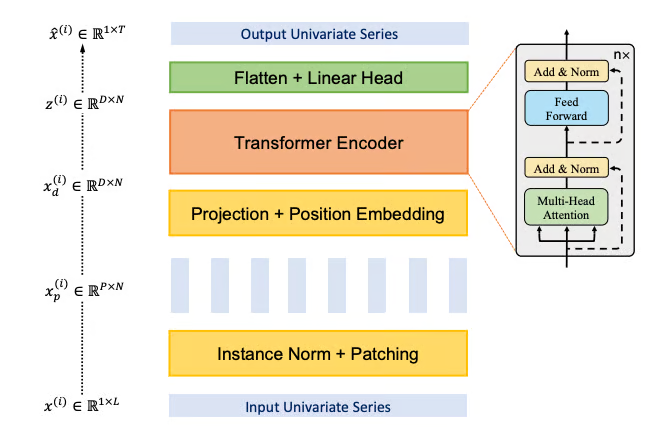
\includegraphics[width=\linewidth,height=54mm,keepaspectratio]{../figures/patchtst.png}
\smallnote{Source: Nie et al., \textit{A Time Series is Worth 64 Words}, ICLR 2023. Same architecture illustration as thesis Chapter 2.}
\column{.36\textwidth}
\small\textbf{Our selected raw model}
\begin{itemize}
\item 30 signal samples; one channel.
\item Patches of 10, stride 2: 11 tokens.
\item Width 128; 4 attention heads; 3 encoder layers.
\item Flatten + linear head: 10 future values at once.
\end{itemize}
\smallnote{The figure shows the original normalization step. Our forecaster has no internal instance normalization: raw or context-standard input is prepared externally.}
\end{columns}
\end{frame}

\begin{frame}[noframenumbering]{B12 | Autoregressive Models: Exact Inputs}
\small $x_t=[S_{t-29},\ldots,S_t]$: one signal channel, sampled every 30 seconds.\par
\vspace{3mm}
\renewcommand{\arraystretch}{1.35}
\begin{tabularx}{\textwidth}{@{}>{\raggedright\arraybackslash}p{59mm}>{\raggedright\arraybackslash}X@{}}
\toprule
Model / task & Input for one prediction\\\midrule
GRU S2V, GRU encoder--decoder, PatchTST & $30\times1$ sequence: $x_t$ or $(x_t-\mu_t)/s_t$. No scalar features.\\
XGBoost / autoregressive & Same 30 raw or standardized lags, flattened. One regressor per future step.\\
Chronos zero-shot & Raw vector of 30 or 120 samples; internal scaling and tokenization.\\
\bottomrule
\end{tabularx}\par
\vspace{3mm}
\textbf{Raw and context-standard are separate runs.}\par
$\mu_t$ and $s_t$ come only from the input window. Standardized forecasts are transformed back with those same statistics.
\smallnote{Shapes exclude the batch dimension. All models output ten future signal values. No scalar summaries, timestamps or meteorological covariates are appended.}
\end{frame}

\begin{frame}[noframenumbering]{B13 | Persistence Models: Exact Inputs}
\small $x_t=[S_{t-29},\ldots,S_t]$,\quad
$r_t=x_t-S_t$,\quad $q_t=x_t-10$.\par
\vspace{3mm}
\renewcommand{\arraystretch}{1.28}
\begin{tabularx}{\textwidth}{@{}>{\raggedright\arraybackslash}p{59mm}>{\raggedright\arraybackslash}X@{}}
\toprule
Model / task & Input for one prediction\\\midrule
Three shapelet models / current-level & $r_t$: $30\times1$ sequence + 12 scalars through a separate embedding.\\
XGBoost / current-level & $[r_t;\,s_t^{\mathrm{CLP}}]$: 42 tabular features.\\
TCN, shapelet convolution / long-fade & $q_t$: $30\times1$ sequence + 14 scalars through a separate embedding.\\
XGBoost / long-fade & $[q_t;\,s_t^{\mathrm{LFD}}]$: 44 tabular features.\\
Selected XGBoost-AFT / survival & 30 raw lags only; no scalar features.\\
Selected TCN / survival & $r_t$: $30\times1$ sequence + 18 scalars through a separate embedding.\\
\bottomrule
\end{tabularx}
\smallnote{Neural models concatenate the scalar embedding with the encoded sequence/shapelets before the output head. Trees concatenate scalar values with lags. Scalar definitions: B14.}
\end{frame}

\begin{frame}[noframenumbering]{B14 | What Is in the Scalar Context?}
\small
\textbf{Ten shared trailing-window summaries}\par\vspace{1mm}
Mean, standard deviation, minimum, maximum and range of the 30 samples;\par
$S_t-S_{t-1}$, $S_t-S_{t-2}$, $S_t-S_{t-4}$; mean and standard deviation of the last five samples.\par
\vspace{3mm}
\renewcommand{\arraystretch}{1.35}
\begin{tabularx}{\textwidth}{@{}>{\raggedright\arraybackslash}p{31mm}>{\raggedright\arraybackslash}X@{}}
\toprule
Task & Added to those ten summaries\\\midrule
Current-level (12) & $S_t$ and $S_t-0.5$: absolute level and level-recovery boundary.\\
Long-fade (14) & $S_t$, $S_t-10$, elapsed event time and observed sample count since onset.\\
Survival TCN (18) & The long-fade feature types, with survival-event onset; plus current threshold status, time since last above-threshold sample, consecutive below-threshold count and above-threshold fraction in the last five event-local samples.\\
\bottomrule
\end{tabularx}
\par\vspace{3mm}
These features restore absolute level and summarize recent changes or event state; they are not extra sensor measurements.
\smallnote{Feature scaling is fitted on training data during selection. No future event end, target duration or censoring label enters the input. Selected AFT does not use this scalar branch.}
\end{frame}
